\subsection{Specific Applications}
\label{subsec:03_applications}

In this section we take a closer look at applications that are linked to cybersecurity on a secondary level: Here the Blockchain is not per se used to mitigate direct cybersecurity threats, but is used to make applications more robust, error-prone and less vulnerable. So the Blockchain does solve cybersecurity related issues, but in a more indirect way.

\subsubsection{Assessment Criteria}
Below we want to introduce multiple different scenarios of applications (existing or proof-of-work drafts) for the Blockchain technology and apart from a brief introduction of the challenges and problems of this specific field, answer the following questions:
\begin{enumerate}
	\item What is the quality of this specific type of application regarding cybersecurity? 
	\item How do they make use of the Blockchain Technology?
	\item Is the BC really needed or could the problems be solved without it? 
\end{enumerate}
To answer question number 3 we are going to make use of the below schema presented by \citeauthor{Wust2017} in \cite{Wust2017}, that helps spliting real use cases from unnecessary ones.
\begin{figure}[ht!]
  \begin{center}
  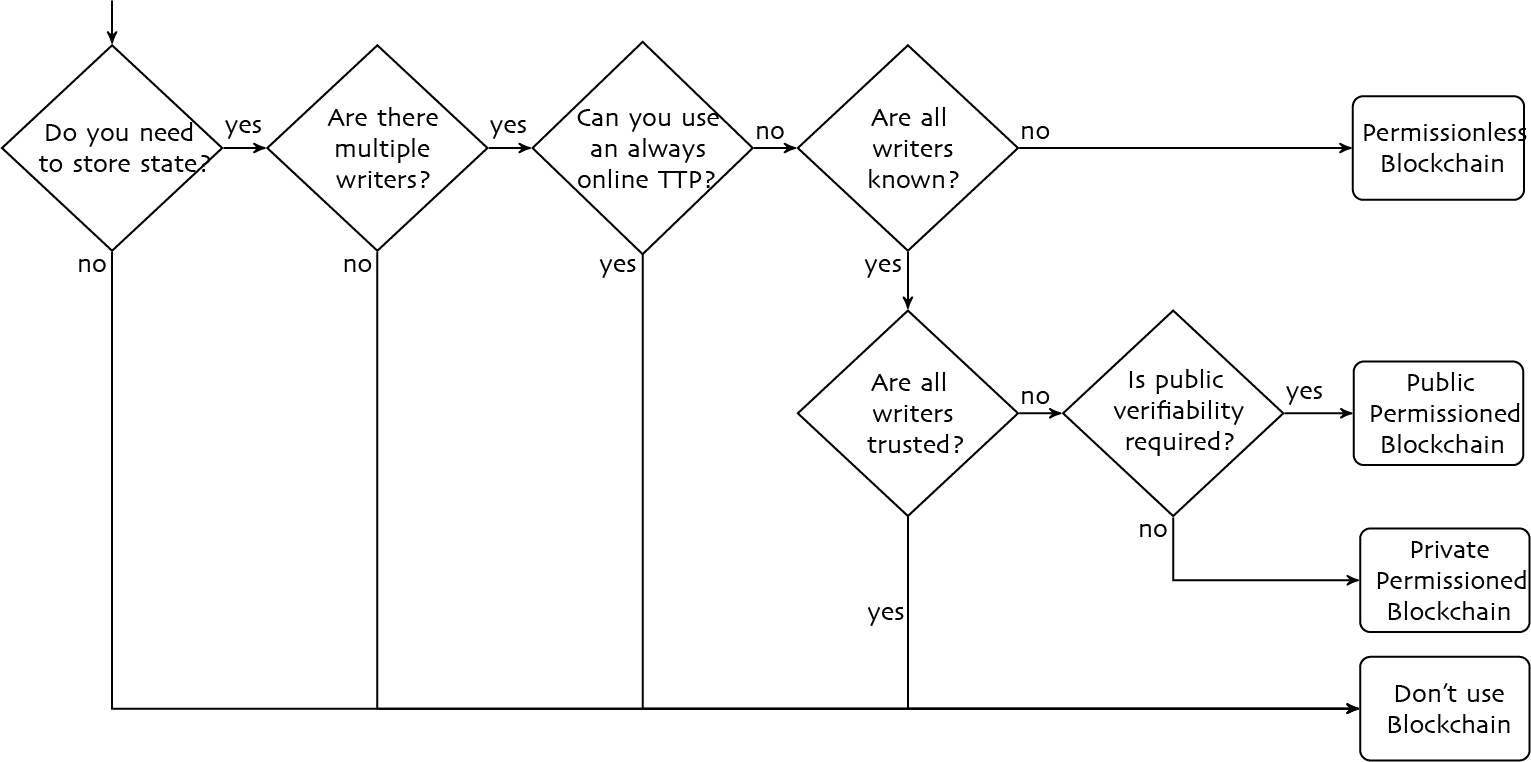
\includegraphics[scale=0.6]{Talk7/img/app/BCorNot}
  \end{center}
  \caption{Do you need a Blockchain?}
  \label{blockchain_or_not}
\end{figure}

\subsubsection{E-Voting}
\begin{itemize}
	\item \cite{Osgood2016}
	\item  \cite{BenAyed2017}
	\item Conclusion by \cite{Wust2017} point F
\end{itemize}
\subsubsection{Autonomous Vehicles}
\begin{itemize}
	\item \cite{Dorri2017}
	\item  \cite{Rowan2017}
	\item \cite{Sharma2017}
\end{itemize}
\subsubsection{Personal Data Protection and Patient Monitoring}
\begin{itemize}
	\item \cite{Zyskind2015}
	\item \cite{Yue2016}
	\item \cite{Azaria2016}
	\item \cite{Fotiou2016}
	\item \cite{Zhang2017}
	\item \cite{Zhang2018}
	\item \cite{Esposito2018}
	\item \cite{Ekblaw2016}
	\item \cite{Cao2019}
\end{itemize}
\subsubsection{Smart Cities \& IoT}
\begin{itemize}
	\item \cite{Biswas2016}
	\item \cite{Mylrea2017}
	\item \cite{Liang2018}
	\item \cite{Dorri2017a}
	\item \cite{Shafagh2017}
\end{itemize}

